\documentclass[final]{beamer}
\mode<presentation>
{\usetheme{Berlin}}

\usepackage[orientation=portrait,size=a0,scale=1.4,debug]{beamerposter}
\usepackage{graphicx}

\title[FastGates]{\huge Next generation platform for implementing fast gates in ion trap quantum computation}
\author[]{\large D. Webb \and O. Bazavan \and S. Saner \and C. Ballance}
\institute[]{\Large
Ion Trap Quantum Computing Group
Department of Physics, University of Oxford}

\begin{document}
\begin{frame}{} 

\maketitle

%%% figs array_sw.png  Figure_2_v2.pdf  setup+beams_horizontal.pdf


\begin{center}

    \begin{block}{}
      XX Shorten Abstract XX\\
    Scalable trapped-ion quantum computation relies on the development of
    high-fidelity fast entangling gates in a many ion
    crystal. Conventional geometric phase gates either suffer from
    scattering errors or off-resonant carrier excitations. A potential
    route to achieve fast entanglement is creating a standing wave which
    can suppress the unwanted carrier coupling [Mundt 2003]. \\

    We present the roadmap to our next-generation platform tailored for
    fast gates in the ~1us regime where gate speeds become comparable to
    the secular trap frequency. The quadrupole transitions between S1/2
    and D5/2 levels in Calcium 40 will be driven to perform
    Molmer-Sorenson gates with a standing wave rather than a typical
    travelling wave. The off-resonant carrier excitation may be strongly
    suppressed by placing ions at the nodes of the optical lattice. This
    new platform has scope for a multi-ion chain and a corresponding array
    of optical lattices which each address a single ion. The lattice array
    is created by a set of counter-propagating beams which are tightly
    focused by a symmetric setup of high-NA lenses. Control of the optical
    phase at the ion site will be achieved by actively stabilising the
    counter-propagating beam interferometer and feedbacking on the ion
    signal.
    \end{block}


\begin{columns}[t]
  \begin{column}{0.49\textwidth}

    \begin{block}{Why Fast Gates?}
      Two qubit gates realised in ion trap QC by coupling spin with motion. Molmer Sorenson interaction achieves this via a bichromatic field incident on the ions:
      $$ \hat{H_{MS}} = \hbar\Omega \hat{S}_{\phi-\pi/2}\cos{(\delta t)} + \hbar\Omega\eta \hat{S}_\phi\cos{(\delta t)}(\hat{a}e^{-i\omega_zt} + \hat{a}^\dagger e^{i\omega_zt})$$
      First term (carrier) a complication whilst second is desired coupling.
      For a quadropole transition, moving into the ??interaction picutre?? this Hamiltonian can be expressed as (modulated by $J_0+J_2$.
      $$ \hat{H_{MS}} = \hbar\eta\Omega(J_0(2\Omega/\delta) + J_2(2\Omega/\delta))\cdot \cos{(\delta t)}\hat{S}_{\phi}(\hat{a}e^{-i\omega_zt} + \hat{a}^\dagger e^{i\omega_zt})$$
      \begin{itemize}
      \item Define a gate - MS hamiltonian
      \item fig: alkali metal zero spin structure diagram
      \item quadropole transition vs Raman

      \item Long coherence time of ions 
      \item Clock speeds of ion trap qc
      \item issues with scaling (commutivity of quadropole MS hamiltionian bessel) and proposed solution
      \item issue with exciting spectators. Use fancy pulse shaping (Vera paper).
      \item fig: pulse shaping
      \item fig: interaction strength with motion saturates.
      \end{itemize}
    \end{block}


    \begin{block}{Fast Gates with a Lattice}
      \begin{itemize}
      \item MS Hamiltionian with lattice removes this saturation.
      \item choosing phase diff of 0 and sitting at antinode to get maximal sb coupling
      \item fig: Control of phase visible to ions
      \item fig: MS gate fidelitly with gate time
      \end{itemize}

      \begin{figure}
        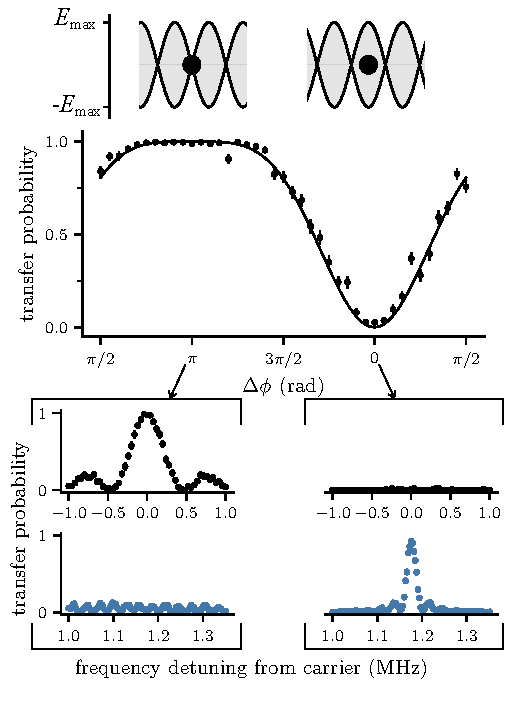
\includegraphics[width=0.5\textwidth]{./figs/Figure_2_v2.pdf}
      \end{figure}

    \end{block}

  \end{column}


  \begin{column}{0.49\textwidth}

    \begin{block}{Phase Stabilization}

      \begin{figure}
        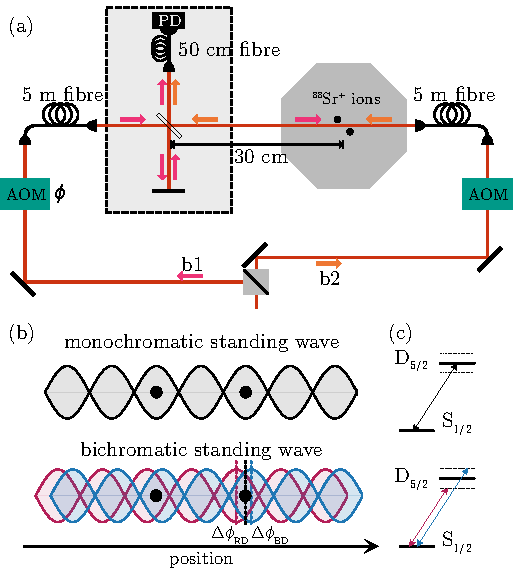
\includegraphics[width=0.5\textwidth]{./figs/setup+beams_horizontal.pdf}
      \end{figure}

      \begin{itemize}
      \item fig: experimental set up (fig1 cnulled)
      \item using ion feedback
      \item fig: RBM data to show no worse
      \end{itemize}
    \end{block}


    \begin{block}{New Platform}
      \begin{itemize}
      \item whats new: double NA, Ca40, NPL trap (3D heating rates), MuMetal shield, perm magnets.
      \item quadropole used.

        ``In practice, the dominant error source in [quadropole] gates is laser
        frequency noise resonant with the carrier transition,
        uncontrolled light shifts arising from the carrier, and laser
        phase noise at time scales comparable with the gate; all of
        these are exacerbated by the relatively small Lamb-Dicke
        parameter (typically ~0.05), which also sets a practical limit
        to the gate speed because it limits gates to the adiabatic
        regime [Roos 2008].''

      \item fig: solidworks of new experiment
      \item fig: array of single addressing SW
      \end{itemize}

      \begin{figure}
        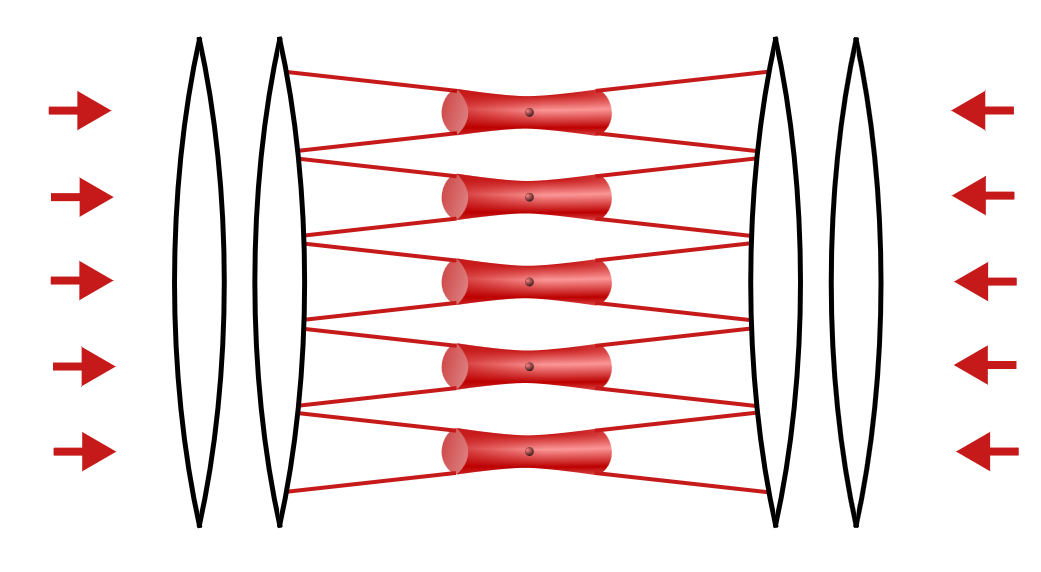
\includegraphics[width=0.75\textwidth]{./figs/array_sw.png}
      \end{figure}

    \end{block}

  \end{column}
\end{columns}
\end{center}

\end{frame}
\end{document}
